\begin{definition}
  For a graded \(k\)-algebra, \(A\), let \(\hinj{\Gr{A}}\) be the full dg-subcategory of \(\CH{\Gr{A}}\) with objects the K-injective complexes of \textcite{Spaltenstein88}. Similarly, we let \(\hinj{\QGr{A}}\) be the full dg-subcategory of \(\CH{\QGr{A}}\) with objects the K-injective complexes.
\end{definition}

\begin{lemma} \label{lemma: omega of Kinj is Kinj}
  The functor 
  \begin{displaymath}
    \omega : \hinj{\QGr{A}} \to \hinj{\Gr{A}}
  \end{displaymath}
  is well-defined. Moreover, \(H^0(\omega)\) is an equivalence with its essential image. 
\end{lemma}

\begin{proof}
  For the first statement, we just need to check that \(\omega\) takes K-injective complexes to K-injective complexes. 
  This is clear from the fact that \(\omega\) is right adjoint to \(\pi\), which is exact.
  
  To see this is fully faithful, we recall that \(\pi \omega \cong \op{Id}\) so
  \[\hinj{\Gr{A}}(\omega M, \omega N) \cong \hinj{\QGr{A}}(\pi\omega M, N) \cong \hinj{\QGr{A}}(M,N).\]
\end{proof}

\begin{remark} \label{remark: enhancement of DQGr}
  Using Lemma~\ref{lemma: omega of Kinj is Kinj}, we can either use \(\hinj{\QGr{A}}\) or its image under \(\omega\) in \(\hinj{\Gr{A}}\) as an enhancement of \(\mathrm{D}(\QGr{A})\). 
\end{remark}

Consider the full dg-subcategory of \(\hinj{\QGr{A \otimes_k B}}\) consisting of the objects
\[\pi_{A \otimes_k B} (A(u) \otimes_k B(v))\]
for all \(u,v\). Denote this subcategory by \(\mathcal E\).

\begin{lemma} \label{lemma: another model for QA otimes QB}
If \(A\) and \(B\) are both Ext-finite, left Noetherian, and right Noetherian, then the dg-category \(\mathcal E\) is naturally quasi-equivalent to \(Q \A \otimes_k Q \B\).
\end{lemma}

\begin{proof}
  Recall that \(Q \A\) is the full dg-subcategory of \(\ldgGrMod{A}\) consisting of \(Q_{A}\) applied to injective resolutions of \(A(u)\), loosely denoted by \(\mathbf{R}Q_A A(u)\), and similarly for \(Q \B\). We have the exact functor
  \begin{displaymath}
    - \otimes_k - : \ldgGrMod{A} \otimes_k \ldgGrMod{B} \to \ldgGrMod{A \otimes_k B}
  \end{displaymath}
  which tensors a pair of modules over \(k\) to yield a bimodule. First consider the triangle
  \begin{gather*}
    \mathbf{R}\tau_{A \otimes B} (\mathbf{R} Q_A A(u) \otimes_k \mathbf{R} Q_B B(v) ) \to \mathbf{R} Q_A A(u) \otimes_k \mathbf{R} Q_B B(v) \\ \to \mathbf{R}Q_{A \otimes B} (\mathbf{R} Q_A A(u) \otimes_k \mathbf{R} Q_B B(v) ).
  \end{gather*}
  By Proposition~\ref{proposition: bi-torsion is a composition}, we have 
  \begin{displaymath}
    \mathbf{R}Q_{A \otimes B} (\mathbf{R} Q_A A(u) \otimes_k \mathbf{R} Q_B B(v) ) \cong \mathbf{R} Q_A \left( \mathbf{R}Q_B \left( \mathbf{R} Q_A A(u) \otimes_k \mathbf{R} Q_B B(v) \right) \right).
  \end{displaymath}
  Since \(\mathbf{R}\tau_B\) commutes with coproducts, we have a natural quasi-isomorphism
  \begin{gather*}
    \mathbf{R} Q_A \left( \mathbf{R}Q_B \left( \mathbf{R} Q_A A(u) \otimes_k \mathbf{R} Q_B B(v) \right) \right) \cong \mathbf{R}Q_A^2 A(u) \otimes_k \mathbf{R}Q_B^2 B(v) \\ \cong \mathbf{R}Q_A A(u) \otimes_k \mathbf{R}Q_B B(v). 
  \end{gather*}
  Thus, 
  \begin{displaymath}
    \mathbf{R} Q_A A(u) \otimes_k \mathbf{R} Q_B B(v) \to \mathbf{R}Q_{A \otimes B} (\mathbf{R} Q_A A(u) \otimes_k \mathbf{R} Q_B B(v) )
  \end{displaymath}
  is quasi-isomorphism for all \(u,v\) with \(\tau_{A \otimes_k B}\) torsion cone. The same consideration shows that the map 
  \begin{displaymath}
    A(u) \otimes_k A(v) \to \mathbf{R} Q_A A(u) \otimes_k \mathbf{R} Q_B B(v)
  \end{displaymath}
  induces a quasi-isomorphism
  \begin{displaymath}
    \mathbf{R}Q_{A \otimes B}( A(u) \otimes_k B(v) ) \to \mathbf{R}Q_{A \otimes B} (\mathbf{R} Q_A A(u) \otimes_k \mathbf{R} Q_B B(v) )
  \end{displaymath}
  with \(\tau_{A \otimes_k B}\) torsion kernel. Now we check that these morphisms induce quasi-isomorphisms on the morphism spaces giving our desired quasi-equivalence. We have a commutative diagram
  \begin{center}
    \scalebox{0.8}{
      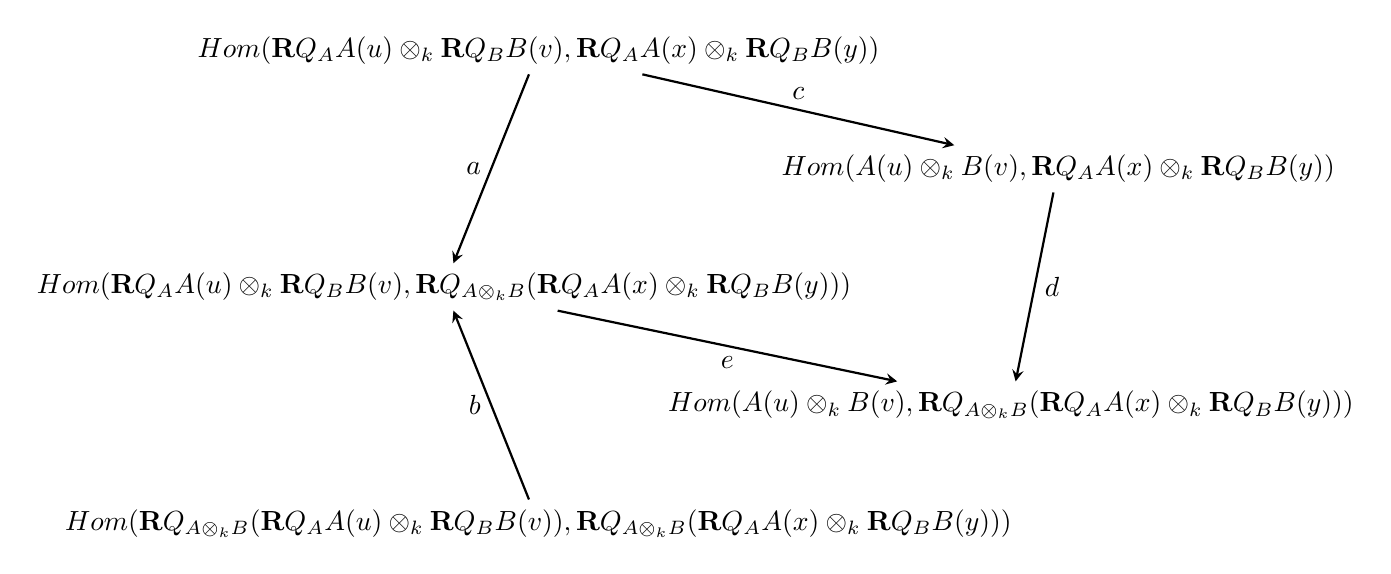
\begin{tikzpicture}[scale=.6,level/.style={->,>=stealth,thick}]
	\node (a) at (-5,5) {\(\op{Hom}(\mathbf{R} Q_A A(u) \otimes_k \mathbf{R} Q_B B(v),\mathbf{R} Q_A A(x) \otimes_k \mathbf{R} Q_B B(y))\)};
	\node (b) at (6,2.5) {\(\op{Hom}(A(u) \otimes_k B(v),\mathbf{R} Q_A A(x) \otimes_k \mathbf{R} Q_B B(y))\)};
	\node (c) at (-7,0) {\(\op{Hom}(\mathbf{R} Q_A A(u) \otimes_k \mathbf{R} Q_B B(v),\mathbf{R}Q_{A \otimes_k B} (\mathbf{R} Q_A A(x) \otimes_k \mathbf{R} Q_B B(y)))\)};
	\node (d) at (5,-2.5) {\(\op{Hom}(A(u) \otimes_k B(v),\mathbf{R}Q_{A \otimes_k B} (\mathbf{R} Q_A A(x) \otimes_k \mathbf{R} Q_B B(y)))\)};
	\node (e) at (-5,-5) {\(\op{Hom}(\mathbf{R}Q_{A \otimes_k B} (\mathbf{R} Q_A A(u) \otimes_k \mathbf{R} Q_B B(v)),\mathbf{R}Q_{A \otimes_k B} (\mathbf{R} Q_A A(x) \otimes_k \mathbf{R} Q_B B(y)))\)};
	\draw[level] (a) -- node[left] {\(a\)} (c) ;
	\draw[level] (e) -- node[left] {\(b\)} (c) ;
	\draw[level] (a) -- node[above] {\(c\)} (b) ;
	\draw[level] (b) -- node[right] {\(d\)} (d) ;
	\draw[level] (c) -- node[below] {\(e\)} (d) ;
    \end{tikzpicture} }
  \end{center}
  and we want to know first that \(a\) and \(b\) are quasi-isomorphisms. We know that \(b\) is a quasi-isomorphism since \(\mathbf{R}\tau_{A \otimes_k B}\) is left orthogonal to \(\mathbf{R}Q_{A \otimes_k B}\) so we only need to check \(a\). Since \(A(u) \otimes_k B(v)\) is free and 
  \begin{displaymath}
    \mathbf{R} Q_A A(u) \otimes_k \mathbf{R} Q_B B(v) \to \mathbf{R}Q_{A \otimes B} (\mathbf{R} Q_A A(u) \otimes_k \mathbf{R} Q_B B(v) )
  \end{displaymath}
  is a quasi-isomorphism, \(d\) is a quasi-isomorphism. Since \(\mathbf{R}Q_A\) and \(\mathbf{R}Q_B\) commute with coproducts, using tensor-Hom adjunction shows that \(c\) is a quasi-isomorphism. Finally, since the cone over the map
  \begin{displaymath}
    A(u) \otimes_k A(v) \to \mathbf{R} Q_A A(u) \otimes_k \mathbf{R} Q_B B(v)
  \end{displaymath}
  is annihilated by \(\tau_{A \otimes_k B}\), we see that \(e\) is also a quasi-isomorphism. This implies that \(a\) is a quasi-isomorphism.
  By an analogous argument, the endomorphisms of \(\mathbf{R}Q_{A \otimes B} (A(u) \otimes_k B(v))\) and \(\mathbf{R}Q_{A \otimes B} (\mathbf{R} Q_A A(u) \otimes_k \mathbf{R} Q_B B(v) )\) are quasi-isomorphic.
\end{proof}



